\setAuthor{Jaan Kalda}
\setRound{lõppvoor}
\setYear{2024}
\setNumber{G 7}
\setDifficulty{7}
\setTopic{TODO}

\prob{Romb}
\begin{wrapfigure}[9]{r}{0.1\textwidth}
  \vspace*{-0mm}
  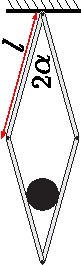
\includegraphics[width = 0.1\textwidth]{2024-v3g-07-yl.pdf}
\end{wrapfigure}
Laest ripub rombikujuline liigendiga konstruktsioon, mis on valmistatud massita varrastest pikkusega $l$, vt joonis. Silinder massiga $m$ pannakse rombi sisse. Selle tulemusel võtab romb tasakaaluasendi, kus rombi tipunurk on $2\alpha$. Hõõrdumine silindri ja varda vahel on tühiselt väike. Leidke silindri raadius.


\hint

\solu
\textit{Lahendus 1}: Vaatleme parempoolse alumise varda tasakaalu, vt joonist. Talle mõjub kokku kolm jõudu. Esiteks on šarniirsesse kinnituspunkti $B$ rakendatud vasakpoolse varda poolt mõjuv jõud, mis on sümmeetria tõttu horisontaalne. Et ülemisele vardale mõjub vaid kaks jõudu (üks ühes otsas ja teine teises otsas), siis peavad need mõlemad olema suunatud piki varrast (vastasel korral ei saaks rahuldada ülemisele vardale mõjuvate  jõumomentide tasakaalutingimust). Seega mõjub alumisele vardale ülemises šarniirses kinnituspunktis jõud, mis on suunatud piki sirget $AC$. Peale selle mõjub alumisele vardale veel silindri toetuspunktis $D$ normaaljõud, mis on suunatud risti vardaga.

Kuivõrd vardaid võib lugeda kaalutuiks, siis varrastele mõjuva raskusjõuga võib mitte arvestada. Kui jäigale kehale on rakendatud vaid kolm jõudu, siis peavad need lõikuma ühes punktis, vastasel korral ei oleks rahuldatud sellele kehale mõjuvate  jõumomentide tasakaalutingimus. Seetõttu peab punkti $D$ rakendatud jõu pikendus läbima punkti $C$. On lihtne näha, et $BC=2l\sin\alpha$, mistõttu $OB=BC\tan\alpha=2l\sin\alpha\tan\alpha$ ning $r=OD=OB\sin\alpha=2l\sin^2\alpha\tan\alpha$.
\begin{center}
  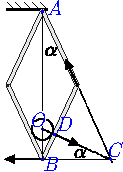
\includegraphics[width=0.3\textwidth]{2024-v3g-07-sol.pdf}
\end{center}

\textit{Lahendus 2}: Silinder avaldab vardale punktis $D$ normaaljõudu $N$. Lisaks mõjub alumisele vardale ülemises šarniirses kinnituspunktis jõud $T$ ülemise varda sihis. Saame kirjutada jõumomentide tasakaalu punkti $B$ suhtes: $N \cdot |BD| =Tl\sin2\alpha$. Jõudude tasakaal silindri jaoks on $2N\sin\alpha=mg$. Jõudude tasakaal punkti $A$ jaoks on $2T\cos\alpha=mg$. Lahendades need kolm võrrandit, saame $|BD|=2l\sin^2\alpha$ ning $r=|BD|\tan\alpha=2l\sin^2\alpha \tan\alpha$.

\textit{Lahendus 3}: Kasutame potentsiaalse energia miinimumi printsiipi: silinder on stabiilselt tasakaalus kui tema masskese on madalaimas võimalikus asendis.

Olgu lae kõrgus $2l$. Silindri keskpunkt asub kõrgusel
\[
  h(\alpha)=2l-2l\cos\alpha + \frac{r}{\sin\alpha}.
\]
Selle tuletis on
\[
  h'(\alpha)=2l\sin\alpha - r\frac{\cos\alpha}{\sin^2\alpha}.
\]
Tingimusest $h'(\alpha)=0$ leiame
\[
  r=2l\frac{\sin^3\alpha}{\cos\alpha}=2l\sin^2\alpha \tan\alpha.
\]
\probend